% ~~~ [ Control Flow Analysis ] ~~~~~~~~~~~~~~~~~~~~~~~~~~~~~~~~~~~~~~~~~~~~~~~~

\subsubsection{Control Flow Analysis}
\label{sec:design_control_flow_analysis}

The key idea behind the control flow analysis (see section \ref{sec:lit_review_control_flow_analysis}), is that high-level control flow primitives may be represented using directed graphs. The problem of structuring low-level code may therefore be rephrased as the problem of identifying subgraphs (e.g. the graph representation of high-level control flow primitives) in graphs (e.g. the CFGs of low-level code) without considering node names, as illustrated in figure \ref{fig:representation_and_identification_of_primitive}. This problem is generally referred to as \textit{subgraph isomorphism search}, which has been well studied \cite{subgraph_isomorphism_algorithms}. Rephrasing the problem in this manner aligns with the design principle of giving each component access to the least amount of information required to successfully accomplish its task. The control flow analysis component is only given access to control flow information (e.g. CFGs), and is oblivious of the underlying LLVM IR. This enables the component to be reused as-is when analysing the control flow of other languages, such as REIL.

\begin{figure}[htbp]
	\centering
	\begin{subfigure}[ht]{0.10\textwidth}
		\lstinputlisting[language=go, style=go, breaklines=false, numbers=none]{inc/primitives/if.c}
		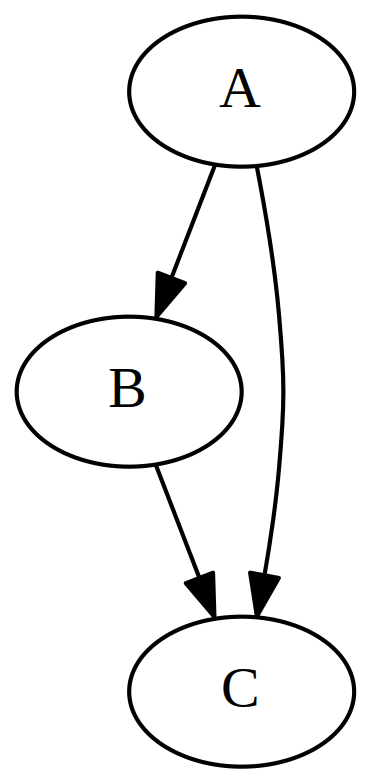
\includegraphics[width=\textwidth]{inc/primitives/if.png}
	\end{subfigure}
	\enskip
	\begin{subfigure}[ht]{0.18\textwidth}
		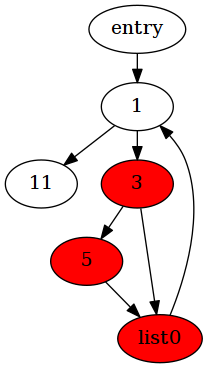
\includegraphics[width=\textwidth]{inc/6_design/example1_highlight.png}
	\end{subfigure}
	\caption{The left side contains the pseudo-code (top left) and graph representation (bottom left) of an if-statement; if \texttt{A} is true then do \texttt{B} followed by \texttt{C}, otherwise do \texttt{C}. The right side highlights (in red) an identified isomorphism of the if-statement's graph representation, in the CFG of the \texttt{main} function presented in appendix \ref{app:clang_example}.}
	\label{fig:representation_and_identification_of_primitive}
\end{figure}

The \texttt{restructure} tool uses subgraph isomorphism search algorithms to locate isomorphisms of the graph representations of high-level control flow primitives in the CFG of a given function. The CFG is simplified by recursively replacing the identified subgraphs with single nodes until the entire CFG has been reduced into a single node; a step-by-step demonstration of which is presented in appendix \ref{app:control_flow_analysis_example}. By recoding the node names of the identified subgraph isomorphisms and the name of their corresponding high-level control flow primitives, a structured CFG may be produced in which all nodes are known to belong to a high-level control flow primitive; as demonstrated in appendix \ref{app:restructure_example}.

The pseudo-code and graph representations of the supported high-level control flow primitives are presented in figure \ref{fig:graph_representations} of section \ref{sec:lit_review_control_flow_analysis}. Should the control flow analysis fail to reduce a CFG into a single node, the CFG is considered irreducible with regards to the supported high-level control flow primitives, in which case a structured CFG cannot be produced.

The \texttt{restructure} tool relies entirely on subgraph isomorphism search to produce structured CFGs (in JSON format) from unstructured CFGs (in the DOT file format). The supported high-level control flow primitives are defined using DOT files, thus promoting a data-driven design which separates data regarding the primitives from the implementation of the \texttt{restructure} tool. A major benefit with this approach is that the \texttt{restructure} tool may search for any high-level control flow primitive that can be expressed in the DOT file format, without any modification to the source code of \texttt{restructure}.

One limitation with this approach is that it does not support graph representations of high-level control flow primitives with a variable number of nodes, as they cannot be described in the DOT file format. For this reason, the \texttt{restructure} tool does not support the recovery of n-way conditionals (e.g. \texttt{switch}-statements). Furthermore, the current design enforces a single-entry/single-exit invariant on the graph representation of high-level control flow primitives. This prevents the recovery of infinite loops, as their graph representation has no exit node. A discussion of how these issues may be mitigated in the future is provided in section \ref{sec:con_design_validation}.
